\chapter{SDN中流量测量sketch的研究现状}

本章将介绍4种典型的用于流量测量的sketch,并分析它们为何无法适用于SDN。

\section{Count-Min\cite{cormode2004improved}}

\begin{figure}[h]
	\centering
	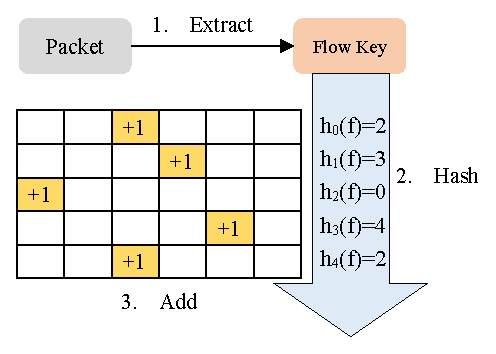
\includegraphics[width=0.8\linewidth]{fig/countmin2.eps}
	\caption{Count-Min的更新过程}\label{fig:countmin}
\end{figure}

如图\ref{fig:countmin}所示,Count-Min sketch的存储形式是一个高度为$d$、长度为$w$的二维数组(也称为\textit{bitmap})。数组中的每个位置称为一个“格子”(slot),格子中包含了一个从0开始的计数器。
数组中的每一行都拥有一个哈希函数,可以将任意流ID,如5元组,映射到$\{0,1,...,w-1\}$之间的某个数。

当一个数据包到达时,Count-Min首先读取它的流ID,然后对于数组的每一行,使用它的哈希函数将ID映射为一个数,用这个数作为索引定位到相应的格子,将格子中的计数器增加。
在统计数据包数的情况下,将计数器加一;在统计数据流量的情况下则将计数器增加相当于数据包字节数的大小。